\documentclass[letterpaper,10pt,twoside,printwatermark=false]{pinp}

%% Some pieces required from the pandoc template
\providecommand{\tightlist}{%
  \setlength{\itemsep}{0pt}\setlength{\parskip}{0pt}}

% Use the lineno option to display guide line numbers if required.
% Note that the use of elements such as single-column equations
% may affect the guide line number alignment.

\usepackage[T1]{fontenc}
\usepackage[utf8]{inputenc}

% The geometry package layout settings need to be set here...
\geometry{layoutsize={0.95588\paperwidth,0.98864\paperheight},%
          layouthoffset=0.02206\paperwidth,%
		  layoutvoffset=0.00568\paperheight}

\definecolor{pinpblue}{HTML}{185FAF}  % imagecolorpicker on blue for new R logo
\definecolor{pnasbluetext}{RGB}{101,0,0} %



\title{DALITE Q1 - Histograms, Medians and Means Solutions.}

\author[a]{EPIB607 - Inferential Statistics}

  \affil[a]{Fall 2018, McGill University}

\setcounter{secnumdepth}{5}

% Please give the surname of the lead author for the running footer
\leadauthor{Bhatnagar and Hanley}

% Keywords are not mandatory, but authors are strongly encouraged to provide them. If provided, please include two to five keywords, separated by the pipe symbol, e.g:
 \keywords{  Histogram |  Density Plot |  Mean |  Median |  Mode  }  

\begin{abstract}
This DALITE quiz will cover the basic concepts of histograms, means and
medians.
\end{abstract}

\dates{This version was compiled on \today}
\doi{\url{https://sahirbhatnagar.com/EPIB607/}}

\pinpfootercontents{DALITE Q1 due Sepetember 12, 2018 by 5pm}

\begin{document}

% Optional adjustment to line up main text (after abstract) of first page with line numbers, when using both lineno and twocolumn options.
% You should only change this length when you've finalised the article contents.
\verticaladjustment{-2pt}

\maketitle
\thispagestyle{firststyle}
\ifthenelse{\boolean{shortarticle}}{\ifthenelse{\boolean{singlecolumn}}{\abscontentformatted}{\abscontent}}{}

% If your first paragraph (i.e. with the \dropcap) contains a list environment (quote, quotation, theorem, definition, enumerate, itemize...), the line after the list may have some extra indentation. If this is the case, add \parshape=0 to the end of the list environment.


\section{Measures of Center Q2}\label{measures-of-center-q2}

The following link
\url{https://www150.statcan.gc.ca/n1/pub/84-537-x/2013005/tbl/tbl1b-eng.htm}
contains the Complete life table for females in Canada from 2009 to
2011. For a given age \(x\), column \(l_x\) gives the number alive (the
cohort starts with 100,000 people) and column \(d_x\) gives the number
of deaths (this column adds up to 100,000 people). The mean age of death
is 83.60. What percentage of people live longer than the mean?

\begin{enumerate}
\def\labelenumi{\alph{enumi})}
\tightlist
\item
  50\%
\item
  \textbf{More than 50\% (Correct)}
\item
  Less than 50\%
\end{enumerate}

\subsection{Correct rationales}\label{correct-rationales}

\begin{itemize}
\tightlist
\item
  At 84 years of age there are 58,833 people alive which is more than
  50\% of the population as the cohort started with 100,000 people.
\item
  At the mean age of death of 83 years old, more than half the
  population (50,000) is still alive.
\item
  Looking at the number of people alive, at 84 we can see that it is
  roughly 58,000. Considering we started with a population of 100,000
  this is more than 50\%.
\end{itemize}

\subsection{Incorrect rationales}\label{incorrect-rationales}

\begin{itemize}
\tightlist
\item
  Because that is the definition of the mean
\item
  The mean is the center of the distribution of deaths. Therefore
  exactly 50\% of people live longer than the mean.
\item
  Usually people live longer than the mean
\item
  Mean represents average value, so if on average people die at 83.6,
  less than 50\% will live after
\end{itemize}

\section{Measures of Center Q3}\label{measures-of-center-q3}

When a group of statisticians from Concordia moved to McGill, they
raised the average intelligence in both universities. Is this possible?
(answer YES or NO and explain).

\begin{enumerate}
\def\labelenumi{\alph{enumi})}
\tightlist
\item
  \textbf{YES (Correct)}
\item
  NO
\end{enumerate}

\subsection{Correct rationales}\label{correct-rationales-1}

\begin{itemize}
\tightlist
\item
  Technically this is possible, if the statisticians have lower
  intelligence than the overall concordia population, and higher
  intelligence than the overall McGill population, they would raise the
  average at both universities.
\item
  If the least smartest statisticians from Concordia became the smartest
  statisticians at another school like McGill, then yes, this is
  possible.
\item
  Yes because of knowledge sharing between the groups from Concordia and
  from McGill. They can then share their new knowledge with their
  respective universities resulting in raising the average intelligence
  in both universities.
\end{itemize}

\subsection{Incorrect rationales}\label{incorrect-rationales-1}

\begin{itemize}
\tightlist
\item
  To raise the intelligence at McGill means that the Concordia
  statisticians must be really smart. If they are really smart, they are
  likely at the top of the distribution of intelligence at Concordia. If
  they leave, they will surely decrease the average.
\item
  The average(mean) is pulled to the lower tail, meaning it is affected
  by the extreme numbers in the dataset. If the average needs to be
  increased, people with relatively high IQ needed to be brought to each
  university.
\item
  Since the number of observations are decreasing in Concordia, average
  intelligence cannot increase in both schools
\end{itemize}

\begin{center}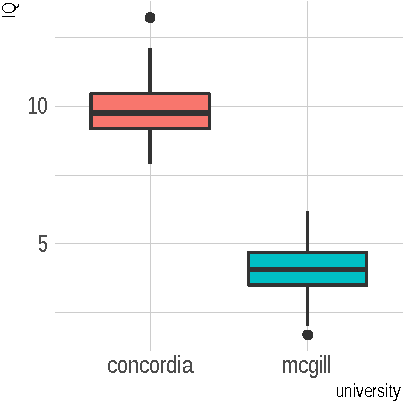
\includegraphics{001-hist-mean-sol_files/figure-latex/unnamed-chunk-2-1} \end{center}

\section{Histograms Q3}\label{histograms-q3}

Six sketches are shown below and labelled (i) to (vi) going from left to
right, top to bottom. Four of them are histograms for the following
variables (in a study of a small town):

\begin{enumerate}
\def\labelenumi{\alph{enumi})}
\tightlist
\item
  heights of all members of households where both parents are less than
  24 years old
\item
  heights of married couples
\item
  heights of all people
\item
  heights of all automobiles
\end{enumerate}

Match each one of the four variables (a)-(d) with the histograms shown
in the figure below.

\begin{enumerate}
\def\labelenumi{\alph{enumi})}
\item
  \begin{enumerate}
  \def\labelenumii{(\alph{enumii})}
  \tightlist
  \item
    -- (iv), (b) -- (ii), (c) -- (iv), (d) -- (i)
  \end{enumerate}
\item
  \begin{enumerate}
  \def\labelenumii{(\alph{enumii})}
  \tightlist
  \item
    -- (ii), (b) -- (iv), (c) -- (i), (d) -- (iv)
  \end{enumerate}
\item
  \textbf{(a) -- (ii), (b) -- (iii), (c) -- (iv), (d) -- (i) (Correct)}
\item
  \begin{enumerate}
  \def\labelenumii{(\alph{enumii})}
  \tightlist
  \item
    -- (ii), (b) -- (vi), (c) -- (v), (d) -- (i)
  \end{enumerate}
\end{enumerate}

\begin{figure}[H]
  \begin{center}
    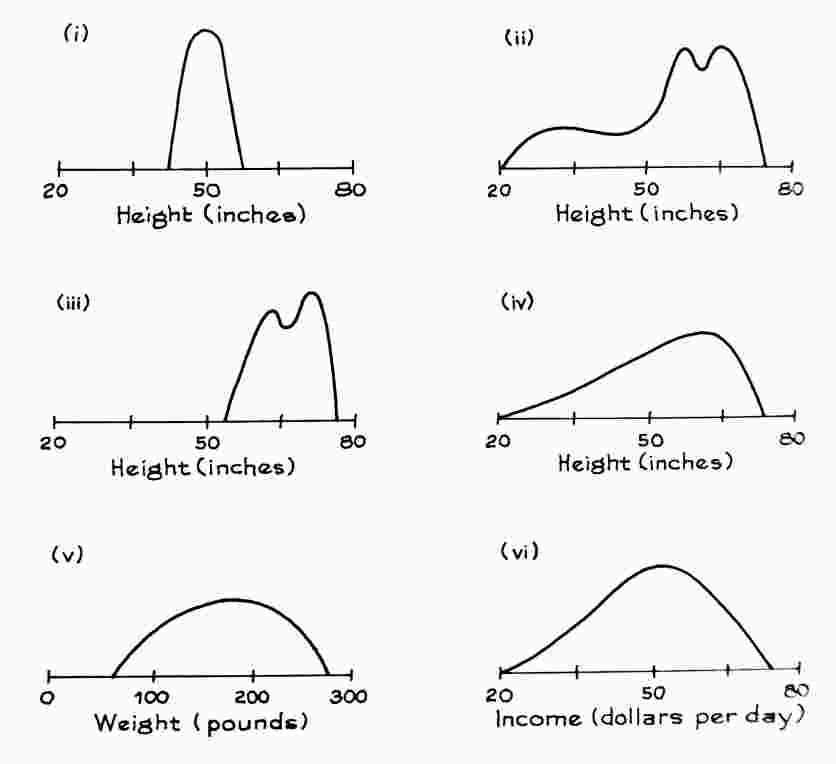
\includegraphics[width=0.66\textwidth, height=3.5in]{hist_q3.jpg} 
  \end{center}
  \caption{Histograms Q3}\label{fig}
\end{figure}

\subsection{Correct rationales}\label{correct-rationales-2}

\begin{itemize}
\tightlist
\item
  Histograms v and vi are irrelevant because of their x-axis variable.
  a(ii) because a there are many differents heights which is expected
  for a family with people from different ages including children.
  b(iii) married couples are adults and on this histogram you only have
  heights above 50 inches. c(iv) is plausible because height in the
  general population should be more of less normally distributed. d(i)
  would be for automobiles because of the narrow range of heights.
\end{itemize}

\subsection{Incorrect rationales}\label{incorrect-rationales-2}

\begin{itemize}
\tightlist
\item
  Heights of all people --\textgreater{} (iv) because it shows the
  incremental growth of the population.
\end{itemize}

\section{Histogram Q2}\label{histogram-q2}

Below are sketches of histograms for test scores in three different
classes. The scores range from 0 to 100; a passing score was 50. For
each class, was the percent who passes about 50\%, well over 50\%, or
well under 50\% ?

\begin{enumerate}
\def\labelenumi{\alph{enumi})}
\item
  \begin{enumerate}
  \def\labelenumii{(\alph{enumii})}
  \tightlist
  \item
    well over 50\%, (b) about 50\%, (c) about 50\%
  \end{enumerate}
\item
  \begin{enumerate}
  \def\labelenumii{(\alph{enumii})}
  \tightlist
  \item
    about 50\%, (b) well under 50\%, (c) about 50\%
  \end{enumerate}
\item
  \textbf{(a) well over 50\%, (b) well under 50\%, (c) about 50\%
  (Correct)}
\item
  \begin{enumerate}
  \def\labelenumii{(\alph{enumii})}
  \tightlist
  \item
    well over 50\%, (b) about 50\%, (c) about 50\%
  \end{enumerate}
\end{enumerate}

\begin{figure}[H]
  \begin{center}
    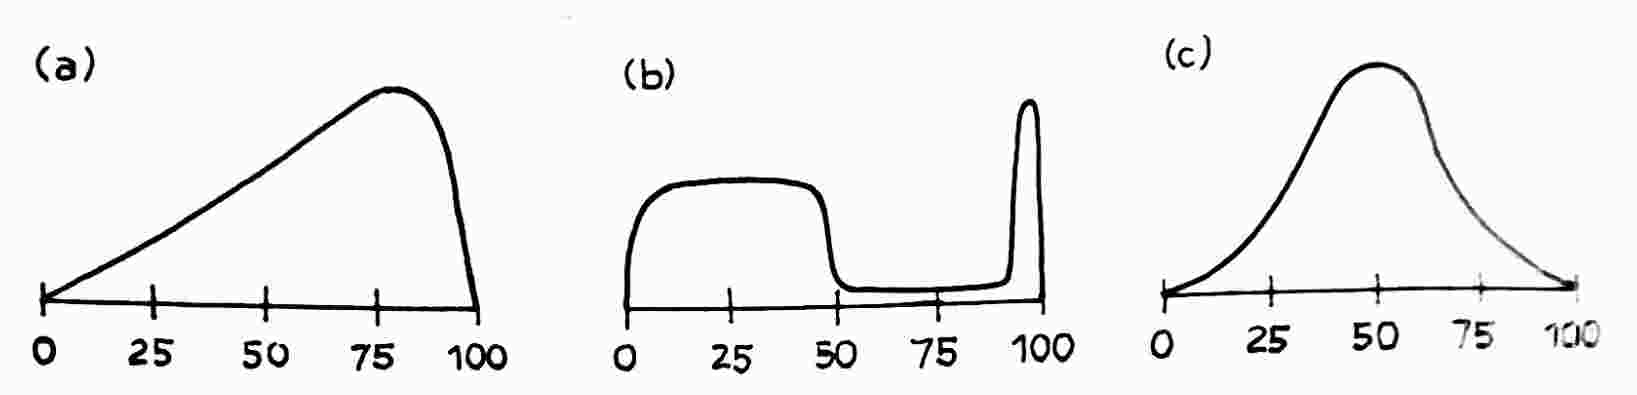
\includegraphics[scale=0.19]{hist_q2.jpg} 
  \end{center}
  \caption{Histogram Q2}\label{fig}
\end{figure}

\subsection{Correct rationales}\label{correct-rationales-3}

\begin{itemize}
\item
  \begin{enumerate}
  \def\labelenumi{(\alph{enumi})}
  \tightlist
  \item
    the density of the plot is greatest above 50, (b) the density of the
    plot is greatest below 50, (c) the density centres around 50
  \end{enumerate}
\item
  a has an area under the curve where more people get higher than 50\% b
  has an area under the curve where more people get lower than 50 \% c
  has an area under the curve where about half of the people get above
  50\% and about half of people get 50\%
\end{itemize}

\subsection{Incorrect rationales}\label{incorrect-rationales-3}

\begin{itemize}
\item
  \begin{enumerate}
  \def\labelenumi{(\alph{enumi})}
  \setcounter{enumi}{1}
  \tightlist
  \item
    high number of people with high scores, so may be about 50
  \end{enumerate}
\item
  \begin{enumerate}
  \def\labelenumi{(\alph{enumi})}
  \setcounter{enumi}{1}
  \tightlist
  \item
    about 50\% there seems to be a high spike of people that got almost
    100 which would bring the \% of people that passed closer to 50\%
  \end{enumerate}
\end{itemize}

\section{Histogram Q1}\label{histogram-q1}

An investigator collects data on hourly wage rates for three groups of
workers. Workers in group B earn about twice as much as those in group
A; workers in group C earn about \$10 an hour more than those in group
A. Which histogram belongs to which group?

\begin{enumerate}
\def\labelenumi{\alph{enumi})}
\tightlist
\item
  \textbf{A(ii), B(i), C(iii) (Correct)}
\item
  A(ii), B(iii), C(i)
\item
  A(i), B(ii), C(iii)
\item
  A(iii), B(i), C(ii)
\end{enumerate}

\begin{figure}[H]
  \begin{center}
    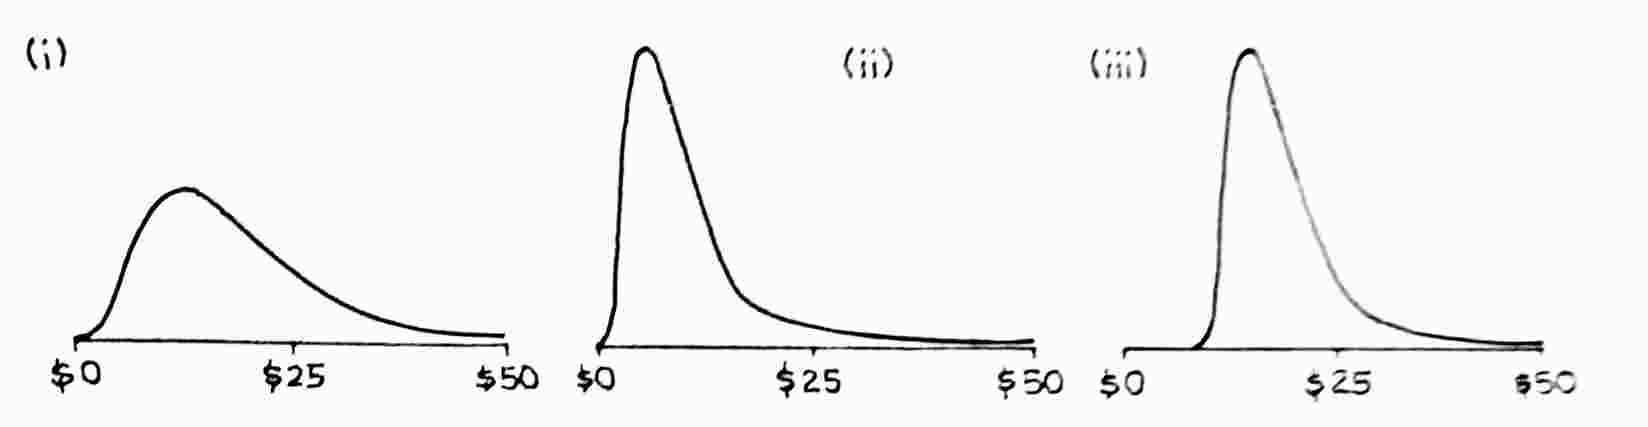
\includegraphics[scale=0.19]{hist_q1.jpg} 
  \end{center}
  \caption{Histogram Q1}\label{fig}
\end{figure}

\subsection{Correct rationales}\label{correct-rationales-4}

\begin{itemize}
\item
  workers in group C earn about \$10 more than A which means that they
  will have the same histogram except it will be shifted \$10 to the
  right
\item
  \begin{enumerate}
  \def\labelenumi{\roman{enumi})}
  \tightlist
  \item
    is group B because the density of the graph is more spread out
    indicating a wider spread of wage. ii) is group A because the
    largest amount of people make the least amount of money. iii) is
    group C because the graph is shifted over to the left indicating the
    the most amount of people make a higher wage than those of group A.
  \end{enumerate}
\end{itemize}

\subsection{Incorrect rationales}\label{incorrect-rationales-4}

\begin{itemize}
\item
  \begin{enumerate}
  \def\labelenumi{(\roman{enumi})}
  \setcounter{enumi}{2}
  \tightlist
  \item
    is shifted to the right therefore workers receive double that of the
    pay of workers in (ii). Using \$25 as a reference point, we find
    that workers in (i) receive more (but not double) that of workers in
    (ii). (i) is also distributed more widely as opposed to having a
    peak.
  \end{enumerate}
\item
  The right shift in the overall histogram (from ii to iii) indicates
  that group B earns twice as much as A.
\item
  Twice as much = histogram higher 10 dollars more = histogram shifted
  away from zero-point
\end{itemize}

\section{Measures of center Q1}\label{measures-of-center-q1}

In a salary dispute involving professional hockey players, the owners
claimed that the average player's salary was \$1 million, while the
players association (NHLPA) said it was `only' \$500k. How can this be?
(assume that these calculations were from the same database)

\begin{enumerate}
\def\labelenumi{\alph{enumi})}
\tightlist
\item
  This is impossible
\item
  The owners were actually talking about the median salary while the
  NHLPA was referring to the mean salary.
\item
  \textbf{The owners were actually talking about the mean salary while
  the NHLPA was referring to the median salary. (Correct)}
\end{enumerate}

\subsection{Correct rationales}\label{correct-rationales-5}

\begin{itemize}
\tightlist
\item
  Some players earn a very large salary, raising the mean, but most
  players earn a more modest salary resulting in the lower median.
\item
  The owners are most likely referring to the mean because the mean
  includes outliers and with a few players in the NHL collecting
  considerably more money, the owners are most likely going to include
  this in their interpretation of the average player salary, which will
  skew the average towards 1 million. On the other hand, the players are
  most likely referring to the median because the probably looked at the
  middle salary entry in the database.
\item
  This is possible as the mean is sensitive to very high/extreme values.
  It is likely that in a sport such as hockey, a small number of players
  are making well above the mean or median which would skew the mean
  value to higher. However because the median simply reports the value
  at which 50\% of players earn more and less, it is not affected by
  what outliers at the top would make. This means that both could be
  right if they used different measures of central tendency
\end{itemize}

\subsection{Incorrect rationales}\label{incorrect-rationales-5}

\begin{itemize}
\tightlist
\item
  The distribution is skewed to the left since hockey players would be
  making top salaries, so it would make sense the the mean is lower than
  the median.
\item
  Since this is a high paying profession, the graph will be skewed to
  the left. This means that the mean is smaller than the median.
  Therefore, it is possible that the players association has the correct
  mean of \$500k, but that the owners who want their players to be paid
  more and would use the median of \$1 million.
\item
  NHLPA was talking about mean/average salary which is lower than the
  median salary (referred by the owners) since few players had
  significantly lower salaries than others which had led to the dispute.
\end{itemize}

%\showmatmethods


\bibliography{pinp}
\bibliographystyle{jss}



\end{document}

